\section{\wasm overview}
\label{sota:wasm}

%\renewcommand{\lstnumberautorefname}{Line}
\newcommand{\lstnumberautorefname}{Line}
\newcommand{\lineref}[1]{\autoref{#1}}


%\todo{Intro}

%\subsection*{}

% Javascript was first, and then more attempts.
Over the past decades, JavaScript has been used in the majority of the browser clients to allow client-side scripting. However, due to the complexity of this language and to gain in performance, several approaches appeared, supporting different languages in the browser.  For example, Java applets were introduced on web pages late in the 90's, Microsoft made an attempt with ActiveX in 1996  and Adobe added ActionScript later on 1998. All these attempts failed to persist, mainly due to security issues and the lack of consensus on the community of browser vendors. 

% asm.js and the demonstration of bad language patterns
In 2014, Emscripten tried with a strict subset of JavaScript, asm.js, to allow low level code such as C to be compiled to JavaScript itself. Asm.js was first implemented as an LLVM backend. This approach came with the benefits of having all the ahead-of-time optimizations from LLVM, gaining in performance on browser clients \cite{asmjs} compared to standard JavaScript code. The main reason why asm.js is faster, is that it limits the language features to those that can be optimized in the LLVM pipeline or those that can be directly translated from the source code. Besides, it removes the majority of the dynamic characteristics of the language, limiting it to numerical types, top-level functions, and one large array in the memory directly accessed as raw data. Since asm.js is a subset of JavaScript it was compatible with all engines at that moment. Asm.js demonstrated that client-code could be improved with the right language design and standarization.
% Limitations o0f asm.js and the birth of Wasm
The work of Van Es \etal \cite{EsAsm.js} proposed to shrink JavaScript to asm.js in a source-to-source strategy, closing the cycle and extending the fact that asm.js was mainly a compilation target for C/C++ code. Despite their result was encouraging, JavaScript faces several limitations related to the intrinsics of the language. For example, any JavaScript engine requires the parsing and the recompilation of the JavaScript code creating overhead.

We, as many in the community consider asm.js the precursor of \wasm. The \wasm (Wasm) language was first publicly announced in 2015. \wasm is a binary instruction format for a stack-based virtual machine and was officially stated later by the work of Haas \etal \cite{Haas_2017} in 2017. The announcement of \wasm marked the first step of standarizing bytecode in the web environment. Wasm is designed to be fast, portable, self-contained and secure, and it outperforms asm.js \cite{Haas_2017}. Since then, the adoption of \wasm has an exponential growth. Cases like the following evidence this fact; Adobe, announced a full online version of Photoshop\footnote{\url{https://twitter.com/Adobe/status/1453034805004685313?s=20&t=Zf1N7-WmzecA0K4V8R69lw}} written in WebAssembly;  game companies moved their development from JavaScript to Wasm like is the case of a fully Minecraft version \footnote{\url{https://satoshinm.github.io/NetCraft/}}; and the case of Blazor \footnote{\url{https://dotnet.microsoft.com/en-us/apps/aspnet/web-apps/blazor}}, a .Net virtual machine implemented in Wasm, able to execute C\# code in the browser.

%\todo{Benchmarks}

\subsection*{From source to Wasm}

All \wasm programs are compiled ahead of time from source languages. LLVM includes Wasm as a target since version 8, supporting a broad range of frontend languages such as C/C++. The resulting binary, works similarly to a shared library, it includes instruction codes, symbols and exported functions. In \autoref{diagrams:sota:wasm}, we illustrate the workflow of the creation of Wasm binaries and their lifecycle. The process starts by compiling the source code program to Wasm (Step \step{1}). To the best of our knowledge, the most complete survey about Wasm tooling is presented in the Awesome Wasm (\url{https://github.com/mbasso/awesome-wasm}) repo. It is a cumulative GitHub repo which includes references to articles, papers, books, demos, compilers and engines related to \wasm. 

The step \step{2} includes the composition of the glue code to Wasm as JavaScript code. This code will include the harness that the Wasm binary needs. For example, by design, Wasm cannot access the DOM of the page as JavaScript code does. In this case, the functions to interact with the DOM are imported in the Wasm binary during its call. The glue JavaScript code can be manually written, however, compilers like Emscripten, Rust and Binaryen can generate it automatically.

Finally, the third step (Step \step{3}), includes the compilation and execution of the client-side code. Most of the browser engines compile either the Wasm code or JavaScript to machine code. In the case of JavaScript this process involves JIT and hot code replacement during runtime. For Wasm, this process is pseudo-direct. For instance, in the case of V8, only two compilation processes are required, a baseline compilation, meant to make the coming binary available as soon as possible and a final one, that makes lane and fast optimizations such as constant folding and dead code removal. This analysis was validated by conversations with the V8 develop team and by one experimental study in our contributions.  

\begin{figure}[h]
    \centering
    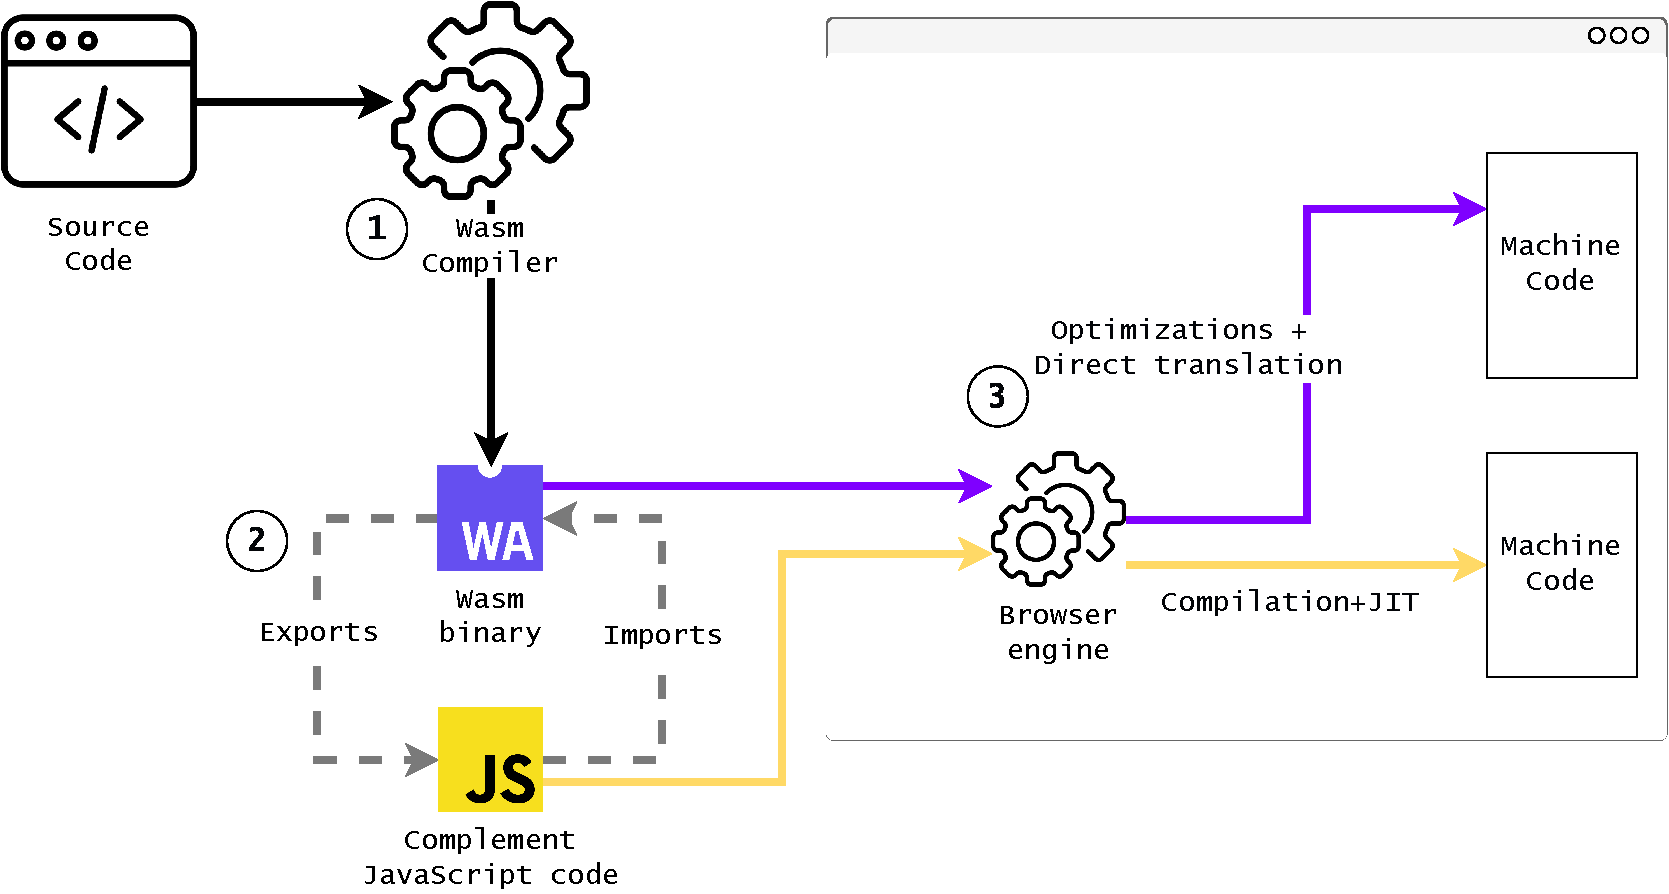
\includegraphics[width=\linewidth]{diagrams/wasm_workflow.pdf}
    \caption{WebAssembly building and lifecycle. }
    \label{diagrams:sota:wasm}
\end{figure}

The Wasm binary might not need external glue code. Thus, depends on the host environment and the binary itself to supply it. This fact encourages the adoption of \wasm further browser engines. For instance, Cloudflare and Fastly adapted their platforms to provide Function as a Service (FaaS) directly with \wasm. In this case the glue code, instead of JavaScript, is provided by any other language stack that the host environment supports.
In 2019, the bytecode alliance team \footnote{\url{https://bytecodealliance.org/}} proposed WebAssembly System Interface (WASI). WASI is the foundation to build Wasm code outside of the browser with a POSIX system interface platform. It standarizes the adoption of \wasm outside web browsers \cite{bryant2020webassembly} in heterogeneous platforms like the Edge or IoT devices \cite{Narayan2021Swivel,Sledge}. 

% Talk about benchmarks and performance numbers

%Previous studies resulted in performance increasing in terms of bandwidth saving, execution, and process-on-demand spawning \cite{9640153, wen2020wasmachine}. The words of Solomon Hykes \footnote{\url{https://twitter.com/solomonstre/status/1111004913222324225}}, the former CEO of docker, show the impact of WASI: 

%\begin{displayquote}
%\textit{
%    If WASM+WASI existed in 2008, we wouldn't have needed to created Docker. That's how important it is. Webassembly on the server is the future of computing. A standardized system interface was the missing link. Let's hope WASI is up to the task!
%}
%\end{displayquote}

%\todo{How to obtain WebAssembly binaries}

%\todo{Browser workflow}

%\todo{How interpreters work, explain the workflow of V8 as it was validated by the V8 compiler developers}

%\todo{Backend workflow}

%\todo{Add a table with tools and interpreters: V8, SpiderMonkey, wasmtime, wasmer, sledge, warduino }


\subsection*{WebAssembly specificities}

% General description and the introduction of the component, module and section terms
\wasm defines its own Instruction Set Architecture (ISA) \cite{wasm_spec}. It is an abstraction close to machine code instructions but agnostic to CPU architectures. Thus, Wasm is platform independent. The ISA of Wasm includes also the necessary components that the binary requires to run in any host engine. 
A Wasm binary has a unique module as its main component. A module is composed by sections, corresponding to 13 types, each of them with an explicit semantic and a specific order inside the module. This makes the compilation to machine code faster. %The binary format of Wasm can include custom sections. For example, the work of \todo{Doe} proposed the usage of custom sections to sign binaries for the sake of trusting. 


% Example and intro to the stack
In \autoref{CExample} and \autoref{WASMExample} we illustrate an arbitrary C code and its compilation to Wasm respectively. The C function contains: head allocation, external function calls and the definition of a function with a loop, conditional branching, function calls and memory accesses. The code in \autoref{WASMExample} is in the textual format for the generated Wasm. The module in this case first defines the signature of the functions(\lineref{tpe1}, \lineref{tpe2}  and  \lineref{tpe3})  that help in the validation of the binary defining its parameter and result types. The information exchange between the host and the Wasm binary might be in two ways, exporting and importing functions, memory and globals to and from the host engine (\lineref{import1}, \lineref{export1} and \lineref{export2}). The definition of the function (\lineref{func1}) and its body follows the last import declaration at \lineref{import1}. 

% Functions
The function body is composed by local variable declarations and typed instructions that are evaluated in a virtual stack (Line 7 to Line 32 in \autoref{WASMExample}). Each instruction reads its operands from the stack and pushes back the result. The result of a function call is the top value of the stack at the end of the execution. In the case of \autoref{WASMExample}, the result value of the main function is the calculation of the last instruction, \texttt{i32.add} at \lineref{result}. A valid Wasm binary should have a valid stack structure that can be verified during its translation to machine code. The stack validation is carried out using the static types of Wasm. 
As the listing shows, instructions are annotated with a type. Wasm binaries contain only four datatypes, \texttt{i32}, \texttt{i64}, \texttt{f32} and \texttt{f64}.

% Example
\begin{code}
    \begin{minipage}[t]{0.4\linewidth}
        \lstset{language=C,caption={Arbitrary C function.},label=CExample,
        escapeinside={(*@}{@*)}
        }
\input{sota/code/code.c}
\end{minipage}\hspace{20mm}
\begin{minipage}[t]{0.4\linewidth}
\lstset{
    language=WAT,
    caption={\wasm code  for \autoref{CExample}.},
    style=WATStyle,
    %stepnumber=0,
    escapeinside={(*@}{@*)},
    numbers=left,
    label=WASMExample}

%
\input{sota/code/code.fix.wat}
%\end{lstlisting}
\end{minipage}


%\begin{tikzpicture}[remember picture,overlay]

%\path (2.west) edge[<-, black] (1.west);
%\path (3.west) edge[<-,  black] (4.west);

%\path (6.east) edge[<-, bend right, black] (3.east);
%\path (9.east) edge[<-, bend right, black] (4.east);
%\path (7.east) edge[<-, bend right, black] (8.east);


%\end{tikzpicture}
\end{code}

% Memory, globals and functions
A Wasm module has a linear memory component that is accessed as \texttt{i32} pointers and should be isolated from the virtual stack. The declaration of the linear data in the memory is showed in \lineref{data}. The memory access is illustrated in \lineref{load}. This memory is usually bound in browser engines to 2Gb of size, and it is only shareable between the process that instantiate the Wasm binary and the binary itself (explicitly declared in \lineref{mem1} and \lineref{export2}). Therefore, this ensures the isolation of the execution of Wasm code. Wasm also provides global variables in their four primitive types. Global variables (\lineref{global1}) are only accessible by their declaration index, and it is not possible to dynamically address them. For function, Wasm follows the same mechanism, either the functions are called by their index (\lineref{call}) or using a static table of function declarations. This latter allows modeling dynamic calls of functions (through pointers) from languages such as C/C++, however, the compiler should populate the static table of functions.


Wasm control flow structures are different to standard assembly programs. All instructions are grouped into blocks, being the start of a function the root block. Two consecutive block declarations can be appreciated in \lineref{block1} and \lineref{block2} of \autoref{WASMExample}. Control flow structures jump between block boundaries and not to any position in the code like regular assembly code. A block may specify the result stack value coming from the execution of its instructions. Inside the Wasm binary the blocks explicitly define where they start and end (\lineref{end1} and \lineref{end2}). Wasm blocks can be, however, by design, each block executes independently and cannot execute or refer to outer block values. This is guarantied by explicitly annotating the state of the stack before and after the block. Three instructions handle the navigation between blocks: unconditional break, conditional break (\lineref{break1} and \lineref{break2}) and table break. Each breaking block instruction can only jump the execution to one of its enclosing blocks. For example, in \autoref{WASMExample}, \lineref{break1} will force the execution to jump to the end of the first block at \lineref{block1} if the value at the top of the stack is greater than zero.

We want to remark that de description of Wasm in this section follows the version 1.0 of the language and not its proposals for extended features. We follow those features implemented in the majority of the vendors according to the Wasm roadmap \cite{wasm_roadmap}. On the other hand we excluded instructions for datatype conversion, table accesses and the majority of the arithmethic instructions for the sake of illustration.

%There are two types of blocks, regular blocks, used to compound pieces of code for stack validation and loops. A loop block manages iterations, the only difference between this to blocks is that the breaking instruction jumps to the end of the block in the case of loops.

% Self contained loops

% Bound memory, no direct access to the DOM

% Roadmap: threads, SIMD, etc

%\todo{Wasm Semantics: Add a code listing, explain General layout of a binary, Function and signature, Instructions, Control flow, Memory model, Global model, table model}

%\todo{Add some sentences from the roadmap}

%\todo{Exported function signature allows typing validation before the code is executed}


\subsection*{WebAssembly's security}

As we described, \wasm is deterministic and well-typed, follows a structured control flow and separate its linear memory model from the program execution stack. This design is robust \cite{WebAssemblySecurity} and makes easy for compilers and engines to sandbox the execution of Wasm binaries.
Host environments should provide protection against common security issues such as data corruption, code injection, and return-oriented programming (ROP). However, WebAssembly is vulnerable under certain conditions, at the execution engine's level \cite{ChromeZero} or the binary itself ~\cite{usenixWasm2020}.
Implementations in both browsers and standalone runtimes~\cite{Narayan2021Swivel} are vulnerable.
This means that if one environment is vulnerable, all the others are vulnerable in the same manner as the same \wasm binary is replicated, turning it into a monoculture problem.

\todo{Extend with our CVE here}

On the other hand, the \wasm environment lacks natural diversity \cite{natural_diversity}. Compared to the work of Harrand \etal \citationneeded, in WebAssembly, one could not use preexisting and different program versions to provide diversification for monoculture solving. In fact, according to the work of Hilbig \etal \cite{Hilbig2021AnES}, the artificial variants created with one of our works contribute to the half of executable and available \wasm binaries in the wild. The current limitations on security and the lack of preexisting diversity motivate our work on software diversification as one possible mitigation among the wide range of security countermeasures. 

\begin{comment}

%\todo{Add example...}
\todo{Go slow...}
\todo{Toolchain, explain frontends, general pipeline...}

In this section, we introduce an overview of the motivation for \wasm and its usage. 
\todo{Jumps to fast, avoid !. Sentece 2} Besides, we describe the process to obtain Wasm programs and how this novel technology evolves from being only-browser-based to standalone executions in the backend. Nevertheless, we describe its significant limitations regarding security, that is our main motivation for our research.

\todo{Why Wasm, asm.js, from source to Wasm, mention benchmarks and examples, photoshop, games, etc, data types, memory model, stack modeling, from Wasm to execution, finalize with security, benefits and limitations. Add diagram}
\todo{The need of a virtual machine or a compiler.}
\todo{Why backend, why WASI as an extension not an essential part of Wasm for the browser.}

\todo{Add diagram, for obtaining Wasm and executing them, with references}
% What is Wasm


% How to generate Wasm code
\wasm binaries are obtained from source code like C/C++ or Rust \cite{Hilbig2021AnES}. The \wasm code is further interpreted or compiled ahead of time into machine code by engines such as the browsers. Since version 8, LLVM supports Wasm as a backend opening the door for its vast collection of frontend languages. The LLVM support was encouraged by the seminal work of Zakai \etal with Emscripten.
Emscripten is an open-source tool for compiling C/C++ to the \wasm. It uses LLVM to create Wasm, but it provides support for faster linking to the object files. Instead of all the IR being compiled by LLVM, the object file is prelinked with Wasm in a faster way. 

\subsection*{\wasm for backend execution}



% Why is important to study Wasm
\subsection*{\wasm security and our motivation for diversification}


\wasm is characterized by a robust security model~\cite{WebAssemblySecurity}. It should run inside a sandboxed execution environment that provides protection against common security issues such as data corruption, code injection, and return-oriented programming (ROP). However, WebAssembly is vulnerable under certain conditions, at the execution engine's level \cite{ChromeZero} or the binary itself ~\cite{usenixWasm2020}.
Implementations in both browsers and standalone runtimes~\cite{Narayan2021Swivel} are vulnerable.
This means that if one environment is vulnerable, all the others are vulnerable in the same manner as the same \wasm binary is replicated, turning it into a monoculture problem.


On the other hand, the \wasm environment lacks natural diversity \cite{natural_diversity}. Compared to the work of Harrand \etal \citationneeded, in WebAssembly, one could not use preexisting and different program versions to provide diversification for monoculture solving. In fact, according to the work of Hilbig \etal \cite{Hilbig2021AnES}, the artificial variants created with one of our works contribute to the half of executable and available \wasm binaries in the wild. 


The current limitations on security and the lack of preexisting diversity motivate our work on software diversification as one possible mitigation among the wide range of security countermeasures. 

\end{comment}
